\documentclass[xcolor={dvipsnames}]{beamer}

\usepackage[english]{babel}
\usepackage[utf8]{inputenc}
\usepackage{times}
\usepackage{amsmath,amsthm, amssymb, latexsym}
\usepackage{rotating}
\usepackage[style=numeric]{biblatex}

\usetheme{Poster}
\usepackage[orientation=portrait,size=a1,scale=1]{beamerposter}

\addbibresource{DanNixon_Poster.bib}

\title{
  The Application of Robust Analysis Methods on Sparse Data for Mass-Resolved
  Neutron Spectroscopy}
\author{Daniel Nixon (120263697) - Supervisor: Paolo Zuliani}

\begin{document}
\begin{frame}{}
  \begin{columns}[t]
    % LEFT COLUMN
    \begin{column}{.49\linewidth}
      \begin{block}{\LARGE Project Aim}
        The aim of this project is to solve two of the current issues relating
        to analysis of data from the VESUVIO spectrometer within the
        Manipulation and Analysis Toolkit for Instrument Data (MANTID)
        \cite{mantid}.
      \end{block}

      \begin{block}{\LARGE Issue 1: Fitting Models}
        \begin{itemize}
            \item Gram-Charlier profile is currently used to fit anisotropic
                  mass peaks (most commonly Hydrogen peaks)
            \item Provides a good level of physical accuracy
            \item Difficult to relate to ab initio results (for example from a
                  simulation)
        \end{itemize}
      \end{block}

      \begin{block}{\LARGE Solution: Multivariate Gaussian model}
        \begin{itemize}
          \item The multivariate Gaussian model can be used as a reasonable
                estimation of the profile of an anisotropic mass peak
          \item Provides a simple means of relating the fitting parameters to ab
                initio calculations
          \item Fitting parameters $\sigma_{x}$, $\sigma_{y}$ and $\sigma_{z}$
                are directly relatable to the dimensions of a momentum ellipsoid
                ($a$, $b$ and $c$ as shown in figure
                \ref{fig:triaxial_ellipsoid}).
        \end{itemize}

        \begin{figure}[h!]
          \centering
          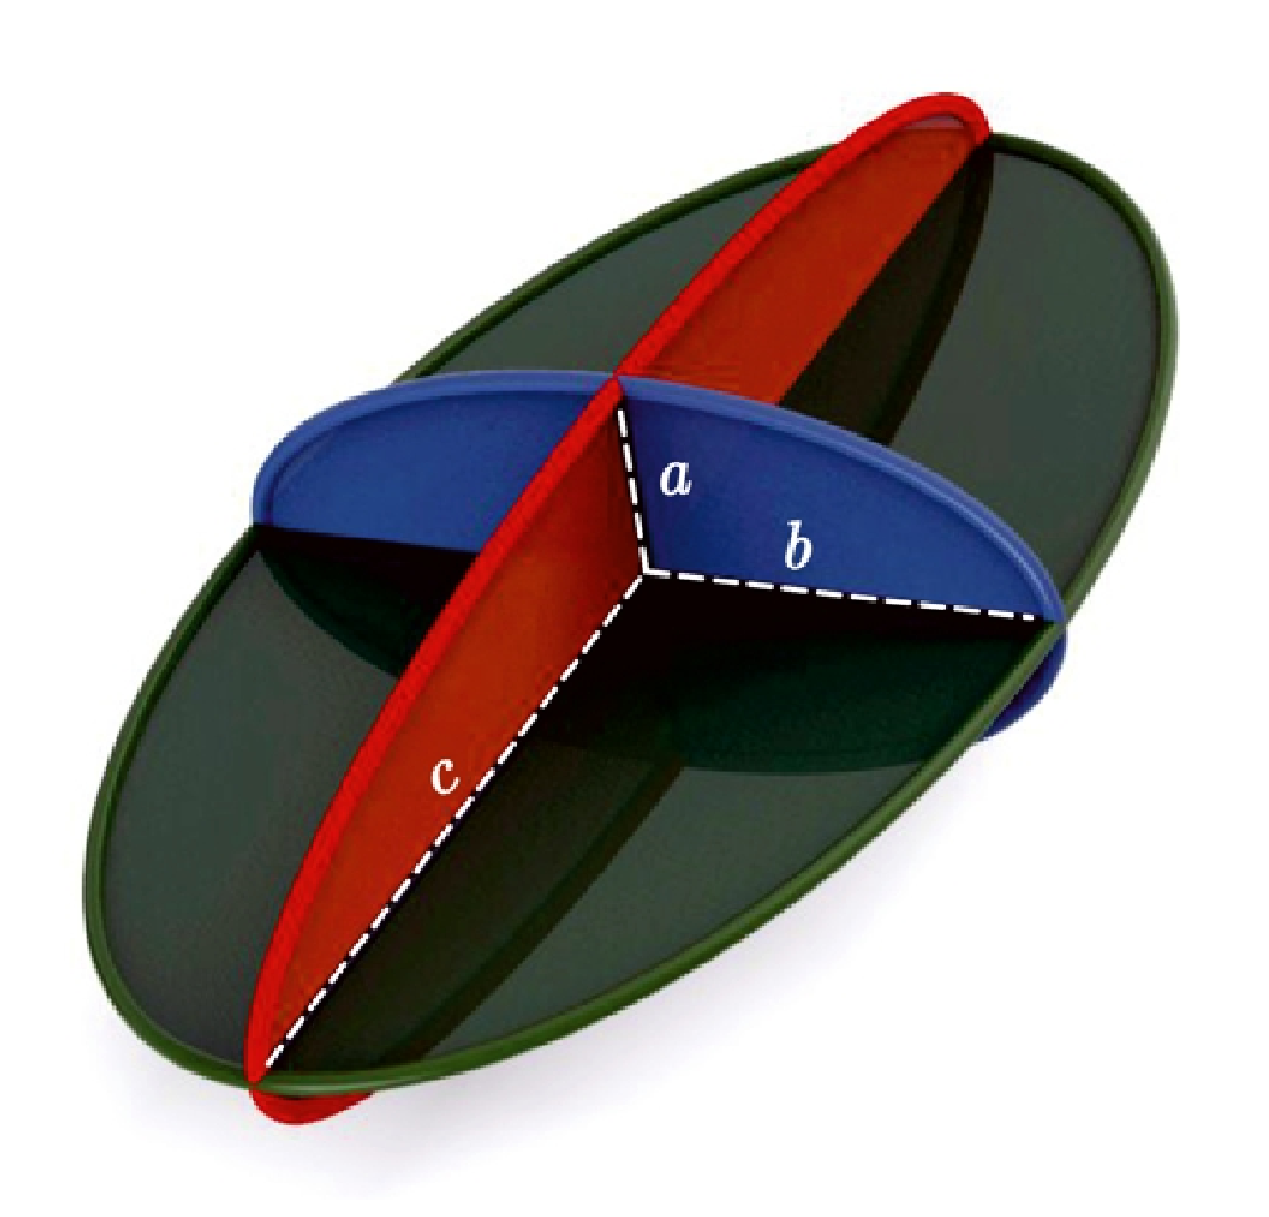
\includegraphics[width=0.4\textwidth]{graphics/Triaxial_Ellipsoid.eps}
          \caption{Triaxial Ellipsoid \cite{ellipsoid}}
          \label{fig:triaxial_ellipsoid}
        \end{figure}

        The multivariate Gaussian model is limited in physical accuracy by the
        accuracy of the numerical integration method implemented, as such is not
        a replacement for the Gram-Charlier profile.
      \end{block}

      \begin{block}{\LARGE Results: Multivariate Gaussian model}
        Ideally the fitted curve of the multivariate Gaussian profile should be
        as close as possible to that of the Gram-Charlier, the fitted curves of
        both models are shown in figure
        \ref{fig:multivariate_gramcharlier_comparison} along with their
        difference.

        \begin{figure}[h!]
          \centering
          \begin{turn}{-90}
            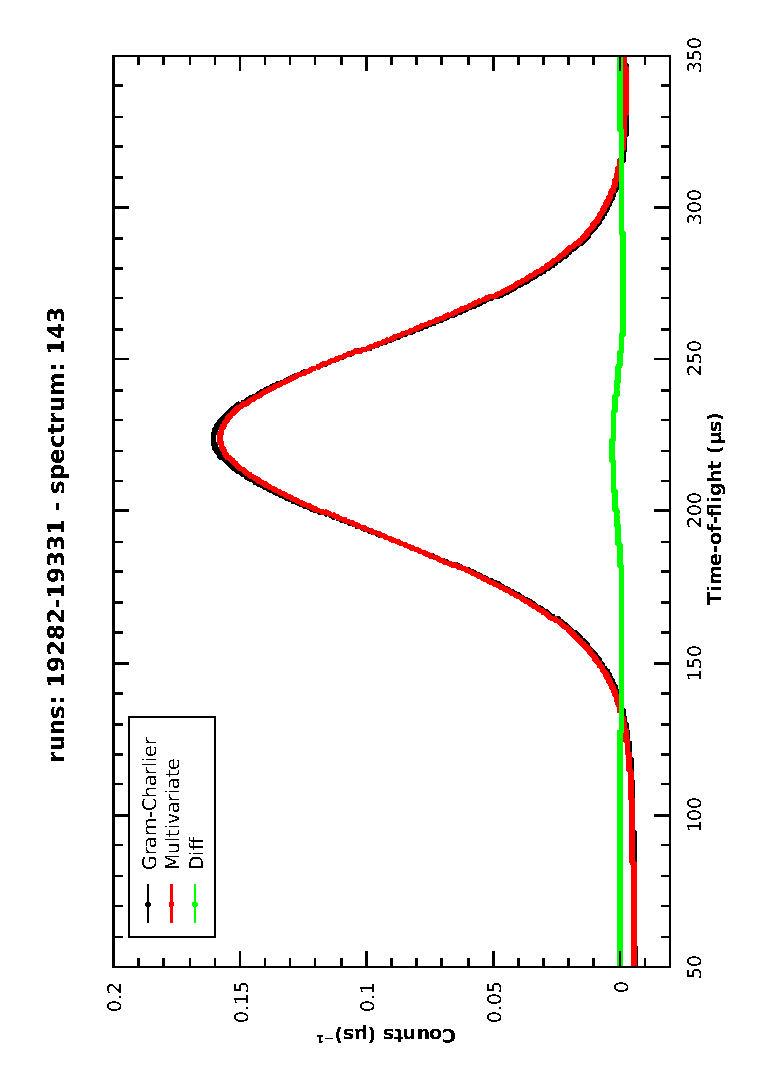
\includegraphics[width=0.6\textwidth]{graphics/multivariate_gramcharlier_comparison.eps}
          \end{turn}
          \caption{Comparison of Gram-Charlier and multivariate Gaussian}
          \label{fig:multivariate_gramcharlier_comparison}
        \end{figure}
      \end{block}
    \end{column}

    % RIGHT COLUMN
    \begin{column}{.49\linewidth}
      \begin{block}{\LARGE Issue 2: Model Selection}
        \begin{itemize}
          \item Current workflow relies on in depth knowledge of the sample
                composition
          \item Increases the time taken in data analysis
          \item Can pose problems when the measured data contains unexpected
                peaks that are not removed or attenuated by an automated
                correction (i.e. container subtraction, gamma background and
                multiple scattering)
        \end{itemize}
      \end{block}

      \begin{block}{\LARGE Solution: Bayesian Model Selection}
        \begin{itemize}
          \item Bayesian model selection provides a simple method of choosing
                the most likely fitting model form a set of possible models
          \item Involves generating a list of possible models by inspecting
                peaks in the measured spectrum to determine what masses could
                contribute to it
          \item For instance the peak in figure
                \ref{fig:majority_overlapping_peaks} has contributions from both
                Carbon and Oxygen
          \item The Fitting Algorithm for Bayesian Analysis of DAta (FABADA)
                \cite{fabada} is then used to select the model that best
                describes the data
        \end{itemize}

        \begin{figure}[h!]
          \centering
          \begin{turn}{-90}
            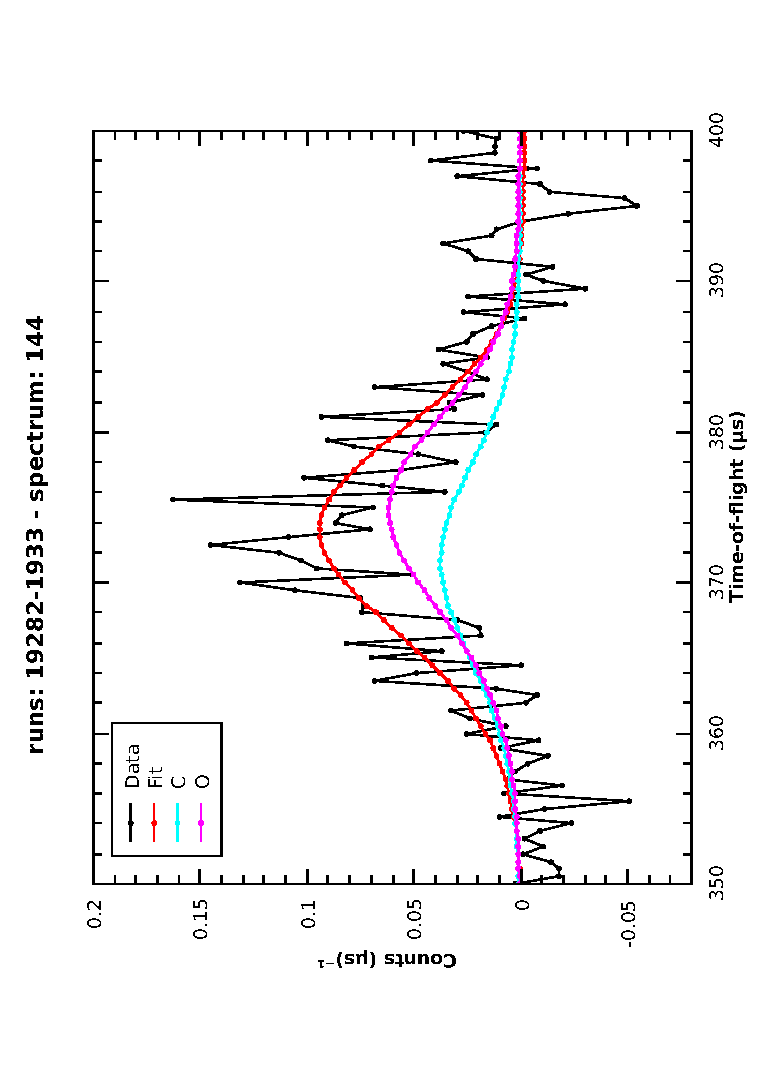
\includegraphics[width=0.55\textwidth]{graphics/majority_overlapping_peaks.eps}
          \end{turn}
          \caption{Example of majority overlapping peaks}
          \label{fig:majority_overlapping_peaks}
        \end{figure}
      \end{block}

      \begin{block}{\LARGE Results: Bayesian Model Selection}
        \begin{itemize}
          \item As it is implemented the model selection routine is not a
                replacement for manual model selection
          \item Has a tendency to misassign peaks when the only prior knowledge
                is the estimates masses as a function of time of flight
          \item Accuracy can be improved by refining the list of possible models
                before the Bayesian selection
          \item Masses that are certainly in the sample can bypass the model
                selection routine (e.g. those that are present in the
                container).
          \item Possible to restrict the possible masses for a peak using
                reduced diffraction data.
        \end{itemize}
      \end{block}

      \begin{block}{\LARGE References}
        \printbibliography
      \end{block}
    \end{column}
  \end{columns}
\end{frame}
\end{document}
